\section{Quantum attack vectors} \label{quantum-attack-vectors}

Quantum attacks refer to attack vectors enhanced by quantum resources, which here we'll refer to as being quantum computational resources.

\subsection{Shor's algorithm} \label{shors-algorithm}

The primary vulnerability current public-key cryptosystems have to quantum attack is via Shor's algorithm for integer factorisation \cite{bib:ShorFactor}. This algorithm has time complexity,
\begin{align}
	O((\log n)^2(\log\log n)(\log\log\log n)),
\end{align}
for an integer of size $n$, and therefore resides in \textbf{BQP} with polynomial quantum time complexity. The quantum circuit implementing Shor's algorithm is shown in Fig.~\ref{fig:shor}.

Recall that the best-known classical algorithm for solving this problem, the general number field Sieve, has time complexity,
\begin{align}
	O(e^{c (\log n)^{1/3}(\log\log n)^{2/3}}),
\end{align}
which is classically inefficient.

A variant of Shor's algorithm can also be used to efficiently solve the discrete logarithm problem, making ECC similarly vulnerable to quantum attack. This arises because, while seemingly very distinct, integer factorisation and the discrete logarithm problem are both closely mathematically related to the problem of period finding.

\begin{figure}[!htb]
\centering
\[
	\Qcircuit @C=.5em @R=.5em {
  \lstick{\ket{0}}    & \gate{H} & \qw & \qw               & \qw               & \qw & \cdots & & \ctrl{4}               & \multigate{3}{\textrm{QFT}_{2n}^{-1}} & \qw  & \meter & \cw \\
  \lstick{\vdots\ \ } & \vdots   &     &                   &                   &     &        & &                        &    \pureghost{\textrm{QFT}_{2n}^{-1}} &      & \vdots &     \\
  \lstick{\ket{0}}    & \gate{H} & \qw & \qw               & \ctrl{2}          & \qw & \cdots & & \qw                    &        \ghost{\textrm{QFT}_{2n}^{-1}} & \qw  & \meter & \cw \\
  \lstick{\ket{0}}    & \gate{H} & \qw & \ctrl{1}          & \qw               & \qw & \cdots & & \qw                    &        \ghost{\textrm{QFT}_{2n}^{-1}} & \qw  & \meter & \cw \\
  \lstick{\ket{1}}    & /^n \qw  & \qw & \gate{U{a^{2^0}}} & \gate{U{a^{2^1}}} & \qw & \cdots & & \gate{U{a^{2^{2n-1}}}} & \qw
 }
 \]
 \caption{Quantum circuit for Shor's algorithm.} \label{fig:shor}
\end{figure}

\subsubsection{How fast is Shor's algorithm in practice?} \label{how-fast-is-shors-algorithm-in-practice}

There is the widely held misconception, often repeated in the mainstream media, that quantum computers could spontaneously crack public key encryption, thereby compromising virtually everything on the internet. In reality, although a Shor-armed quantum computer could `efficiently' crack RSA/ECC cryptography (in the computer scientist's sense of the word `efficient'), it would still take considerable time.

The quantum circuit itself for implementing Shor's algorithm is, despite being efficient, very complex, comprising a large number of quantum gates for realistic problem instances, and requiring elaborate error-correction codes to enable fault-tolerance, inducing significant additional overheads.

(??? Steal figures and results from Brennan/Tomamichel)

\subsection{Grover's algorithm}\label{grovers-algorithm}

Grover's algorithm \cite{bib:Grover96} is a quantum algorithm for speeding up \emph{satisfiability problems}. Suppose we have an arbitrary binary circuit with $n$ input bits and a single output bit, and our goal is to find an input bitstring that evaluates to 1 at the output. We say that the corresponding input is a \emph{satisfying input}. Next, suppose there is only one satisfying input and our goal is to find it (see Fig.~\ref{fig:SAT}).

Classically, without knowing anything about the structure of the circuit, the best we could do is exhaustively search the input space, of which there are $2^n$ combinations. This is referred to as an \emph{unstructured search problem}. The classical runtime, therefore, scales as $O(2^n)$.

Grover's algorithm (ignoring any architectural or fault-tolerance overheads) provides a quadratic enhancement to this, yielding a quantum runtime of only,
\begin{align}
    O(\sqrt{2^n}) = O(2^{n/2}).
\end{align}
The circuit implementing Grover's algorithm is shown in Fig.~\ref{fig:grover}.

\begin{figure*}[!htb]
	\centering
	\[]
	 \Qcircuit @C=1em @R=.7em {
                   &         &                      &                         &                      & \ustick{\text{Grover diffusion operator}} \\
  \lstick{\ket{0}} & /^n \qw & \gate{H^{\otimes n}} & \multigate{1}{U_\omega} & \gate{H^{\otimes n}} & \gate{2 \ket{0^n}\bra{0^n} - I_n}         & \gate{H^{\otimes n}} & \qw & \cdots & & \meter & \cw \\
  \lstick{\ket{1}} & \qw     & \gate{H}             & \ghost{U_\omega}        & \qw                  & \qw                                       & \qw                  & \qw & \cdots & \\
                   &         &                      &                         &                      & \dstick{\text{Repeat $O(\sqrt{N})$ times}}
  \gategroup{2}{5}{2}{7}{.7em}{^\}}
  \gategroup{2}{4}{3}{10}{.7em}{_\}}
 }
 \]
\caption{Quantum circuit for Grover's algorithm.} \label{fig:grover}	
\end{figure*}

We see that Grover's algorithm does \emph{not} provide an exponential quantum speedup, only a quadratic one. From a runtime perspective, this means Grover's algorithm effectively halves the size of the input bit-string.

\begin{figure}[!htb]
	\centering
	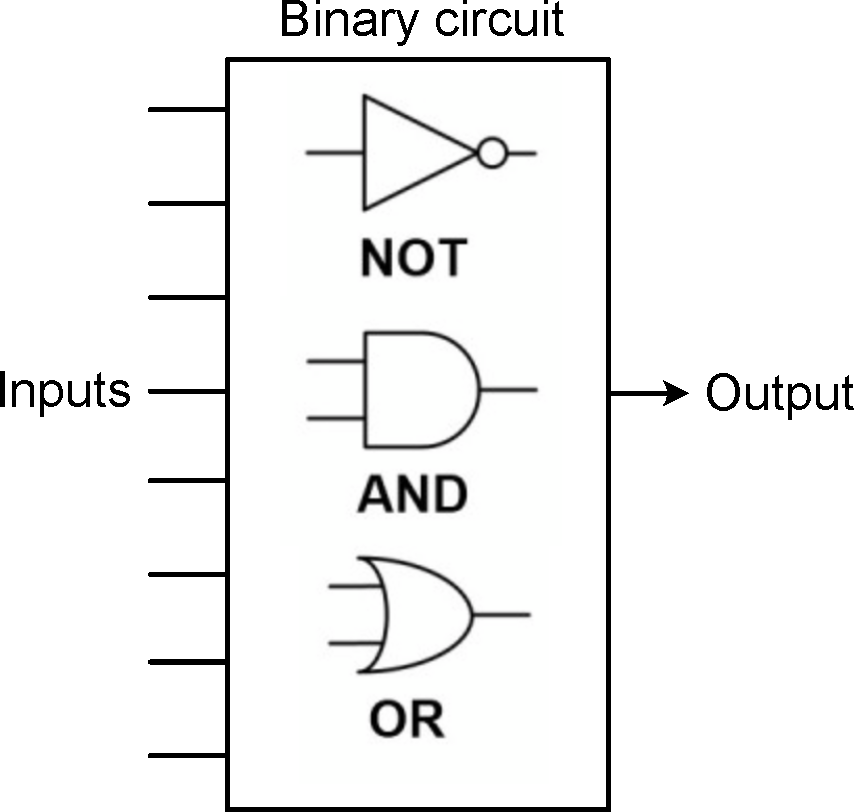
\includegraphics[width=0.7\columnwidth]{figures/SAT}
	\caption{A binary satisfiability problem. A circuit comprising universal binary logic gates (e.g AND, OR and NOT) is applied to an arbitrarily sized input to yield a single output bit. The goal is to find a `satisfying input' such that the respective output yields a 1.} \label{fig:SAT}
\end{figure}

Breaking \emph{any} encryption scheme, private or public, can be viewed as a satisfiability problem, where we ask the satisfiability question ``What key decrypts this ciphertext to something sensible?''. The exception to this is the one-time-pad, since there are keys that decrypt any given message to \emph{every} possible plaintext of the same length, all of which meet the satisfiability criteria.

Similarly, inverse hashing also takes the form of a satisfiability problem, where we want to find an input that maps to a given output. Using Grover's algorithm inverse hashing remains an exponentially hard problem on quantum computers, just a quadratically reduced exponential.

In the quantum era it will therefore be diligent to use private keys and cryptographic hashes of twice the length of what is presently considered secure in order to maintain the same level of security. These are relatively straightforward transitions to make, but ones worth considering implementing today for information with forward value.

\subsection{Symmetric ciphers} 

???

Some, but not all, symmetric ciphers are also vulnerable to efficient quantum attacks via Simon's period finding algorithm. Simon's problem can be stated as follows. For a binary function,
\begin{align}
f: \{0,1\}^n \to \{0,1\}^n,
\end{align}
which satisfies,
\begin{align}
f(x) = f(x\oplus s)	
\end{align}
for some value of $s$ (not including the trivial case where $s=0^n$), where $x,s\in \{0,1\}^n$, the goal is to determine $s$ by querying $f(x)$. Here, $s$ is referred to as the \emph{period} of the function.

The best classical algorithm for solving this problem requires $O(\sqrt{2^n})$ queries, whereas Simon's quantum algorithm requires only $O(n)$ queries, providing an exponential separation between Simon's algorithm and the best classical algorithm. The quantum circuit implementing Simon's algorithm is shown in Fig.~\ref{fig:simons}.

\cite{bib:kaplan2016breaking}

% https://link.springer.com/content/pdf/10.1007/978-3-662-53008-5_8.pdf
% https://en.wikipedia.org/wiki/Slide_attack

\begin{figure}[!htb]
\centering
\[
 \Qcircuit @C=1em @R=.7em {
  \lstick{\ket{0}} & /^n \qw & \gate{H^{\otimes n}} & \multigate{1}{U_f} & \gate{H^{\otimes n}} & \meter & \cw \\
  \lstick{\ket{0}} & /^n \qw & \qw                  & \ghost{U_f}        & \qw                  & \meter & \cw
  }
 \]
 \caption{Quantum circuit for Simon's algorithm.} \label{fig:simons}
\end{figure}